\begin{figure}[t!]
	\centering
	\begin{subfigure}[b]{0.2175\textwidth}
		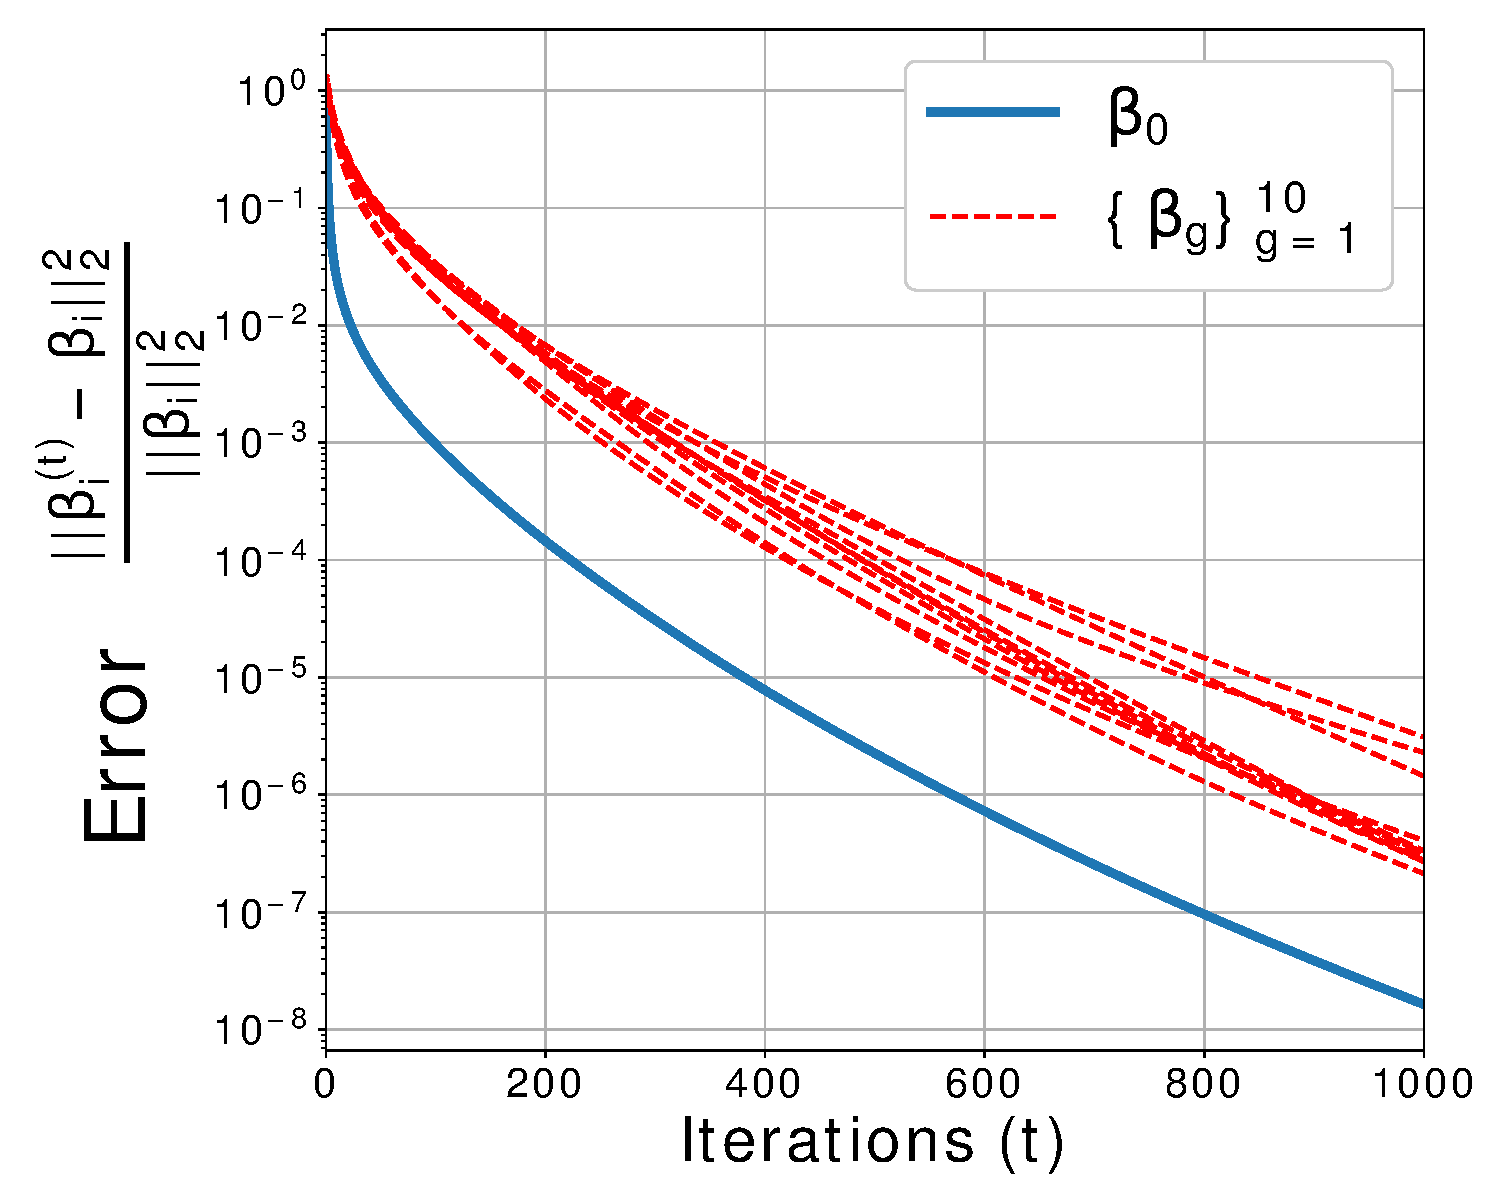
\includegraphics[width=\textwidth]{./img/betag_converge_G10_p100.pdf}				
		\caption{}\label{fig syn1a}
	\end{subfigure} ~
	\begin{subfigure}[b]{0.2175\textwidth}
		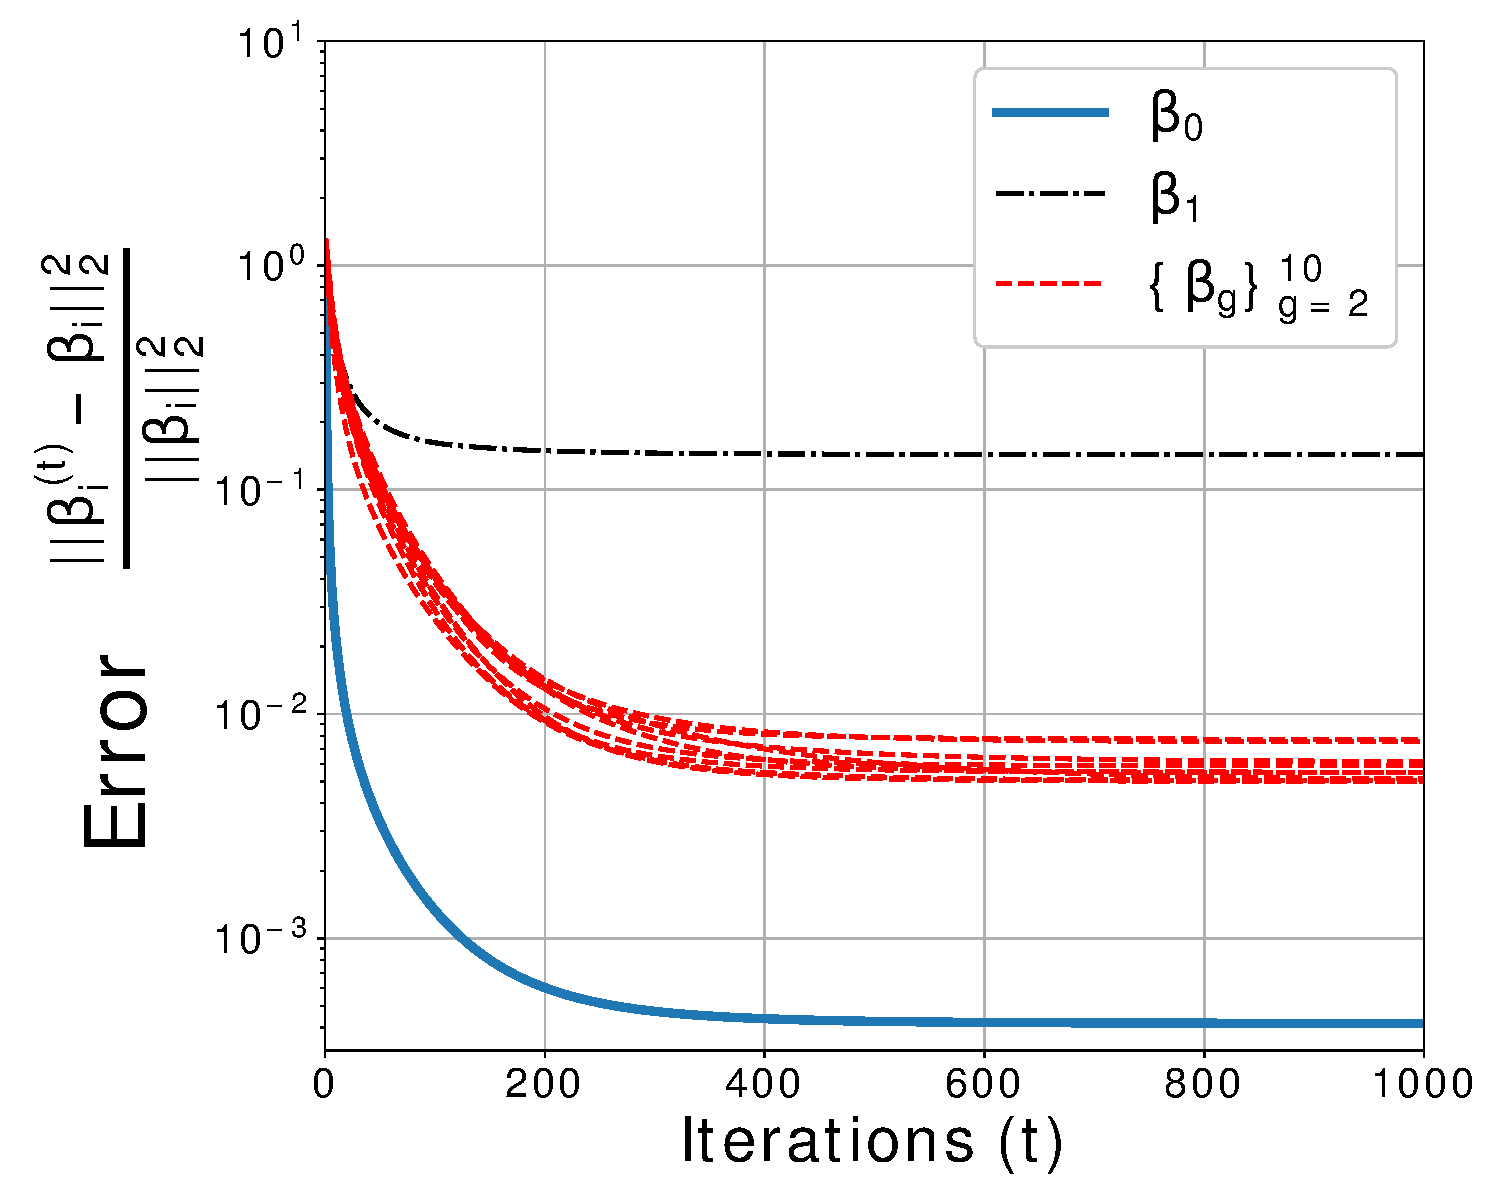
\includegraphics[width=\textwidth]{./img/betag_converge_noise_G10_p100.pdf}				
		\caption{}\label{fig syn1b}
	\end{subfigure}
	%			\label{fig syn1}
	\begin{subfigure}[b]{0.2175\textwidth}
		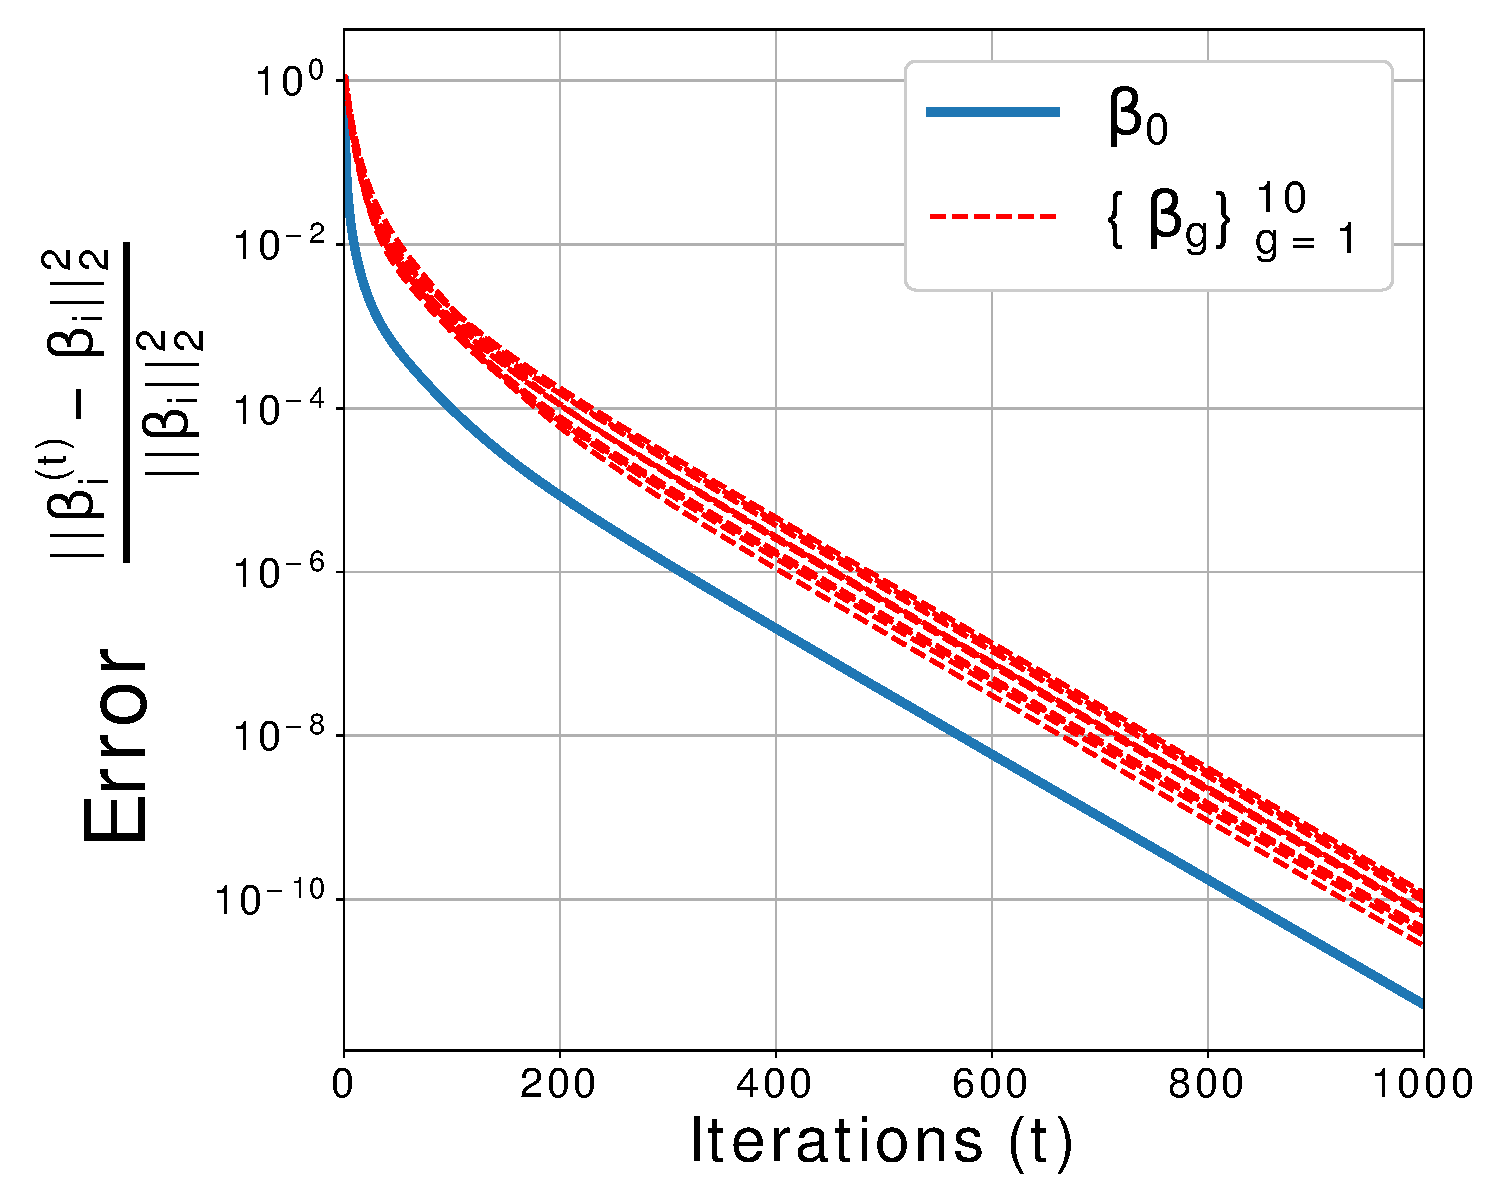
\includegraphics[width=\textwidth]{./img/betag_converge_G10_p100_fast.pdf}
		\caption{} \label{fig syn2a}
	\end{subfigure} ~
	\begin{subfigure}[b]{0.2175\textwidth}
		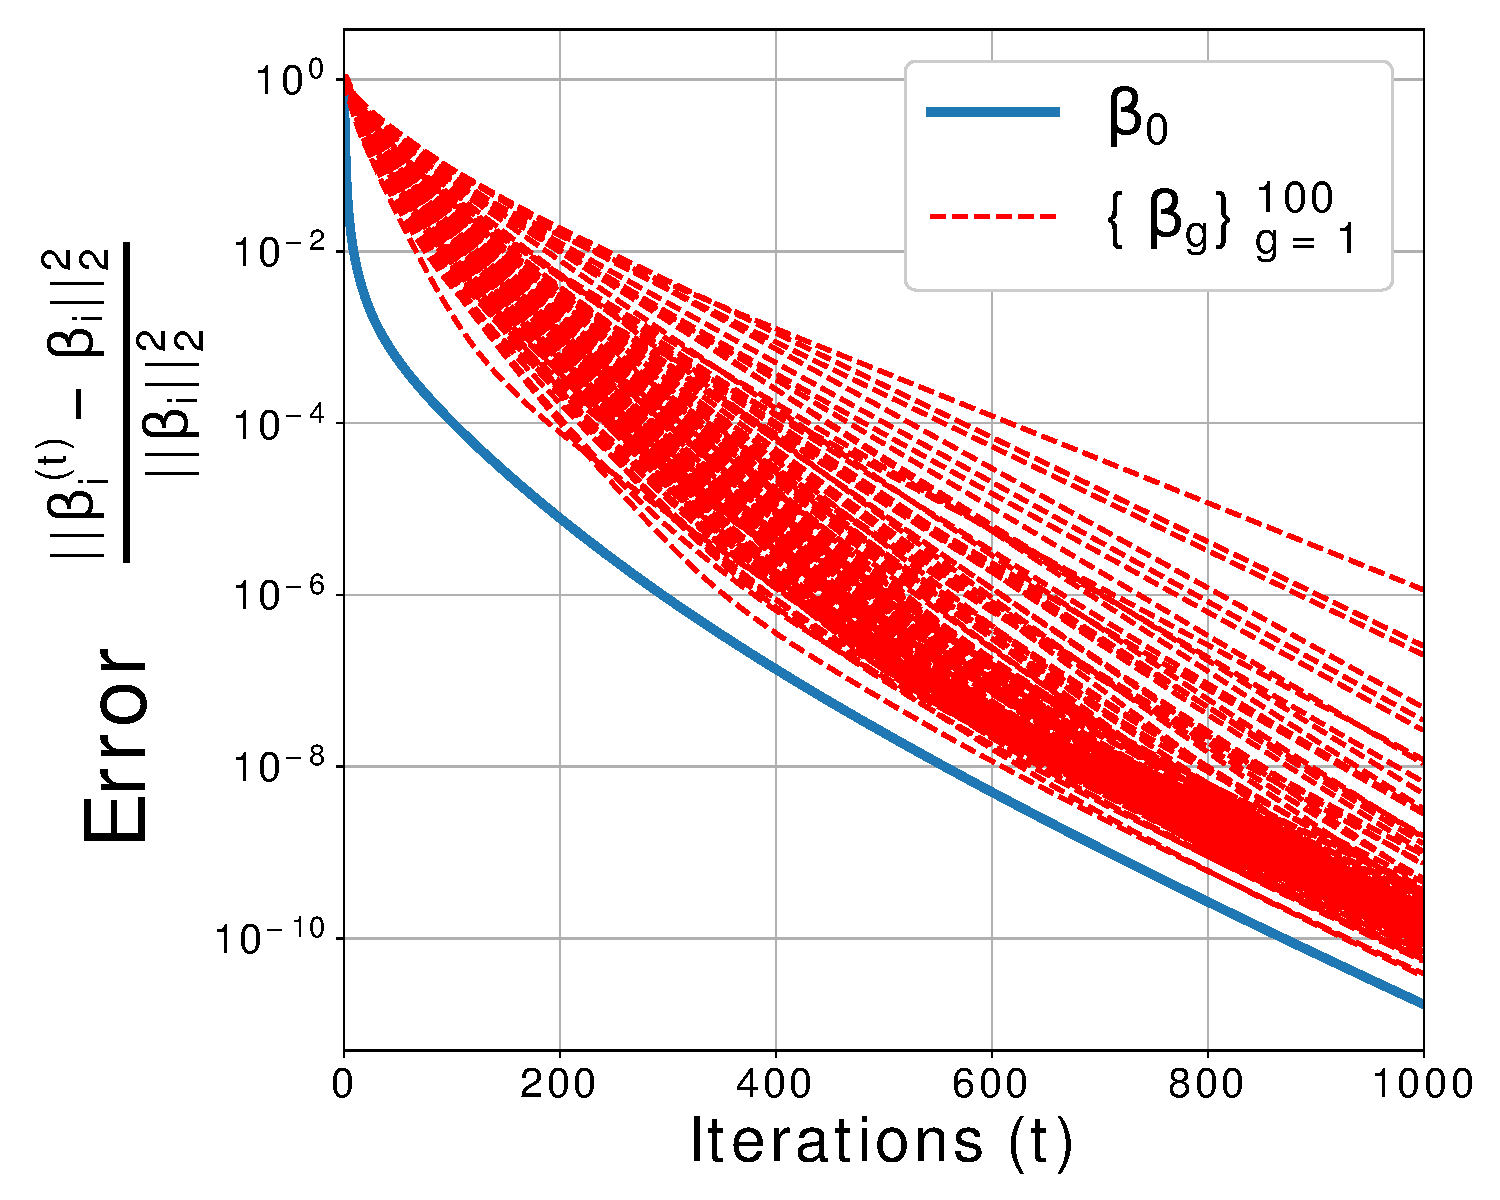
\includegraphics[width=\textwidth]{./img/betag_converge_G100_p1000_shrink.pdf}
		\caption{}\label{fig syn2b}
	\end{subfigure}
	\squeezeup
	\caption{a) Noiseless fast convergence. b) Noise on the first group does not impact other groups as much. c) Increasing sample size improves rate of convergence. d) Our algorithm convergences fast even with a large number of groups $G=100$.}
	\label{fig syn12}
\end{figure}
\section{Synthetic Experiments}
\label{sec:expds}
We considered sparsity based simulations with varying $G$ and sparsity levels. In our first set of simulations, we set $p=100$, $G=10$ and sparsity of the individual parameters to be $s=10$. We generated a dense $\bbeta_0$ with $\|\bbeta_0\|=p$ and did not impose any constraint. Iterates $\{\bbeta^{(t)}_g\}_{g=1}^G$ are obtained by projection onto the $\ell_1$ ball $\|\bbeta_g\|_1$. Nonzero entries of $\bbeta_g$ are generated with ${\cal{N}}(0,1)$ and nonzero supports are picked uniformly at random. Inspired from our theoretical step size choices, in all experiments, we used simplified learning rates of $\frac{1}{n}$ for $\bbeta_0$ and $\frac{1}{\sqrt{nn_g}}$ for $\bbeta_g$, $g \in [G]_\setminus$. Observe that, cones of the individual parameters intersect with that of $\bbeta_0$ hence this setup actually violates DERIC (which requires an arbitrarily small constant fraction of groups to be non-intersecting). Our intuition is that the individual parameters are mostly incoherent with each other and the existence of a nonzero perturbation over $\bbeta_g$'s that keeps all measurements intact is unlikely. Remarkably, experimental results still show successful learning of all parameters from small amount of samples. We picked $n_g=60$ for each group. Hence, in total, we have $11p=1100$ unknowns, $200=G\times 10+100$ degrees of freedom and $G\times 60=600$ samples. In all figures, we study the normalized squared error $\frac{\|\bbeta^{(t)}_g-\bbeta_g\|_2^2}{\|\bbeta_g\|_2^2}$ and average $10$ independent realization for each curve. \cref{fig syn1a} shows the estimation performance as a function of iteration number $t$. While each group might behave slightly different, we do observe that all parameters are linear converging to ground truth.% is evident from the linear slope of the $y$-axis.
	
In \cref{fig syn1b}, we test the noise robustness of our algorithm. We add a ${\cal{N}}(0,1)$ noise to the $n_1=60$ measurements of the first group \emph{only}. The other groups are left untouched. While all parameters suffer nonzero estimation error, we observe that, the global parameter $\bbeta_0$ and noise-free groups $\{\bbeta_g\}_{g=2}^G$ have substantially less estimation error. This implies that noise in one group mostly affects itself rather than the global estimation. In \cref{fig syn2a}, we increased the sample size to $n_g=150$ per group. We observe that, in comparison to \cref{fig syn1a}, rate of convergence receives a boost from the additional samples as predicted by our theory.
	
	
Finally, \cref{fig syn2b} considers a very high-dimensional problem where $p=1000$, $G=100$, individual parameters are $10$ sparse, $\bbeta_0$ is $100$ sparse and $n_g=150$. The total degrees of freedom is $1100$, number of unknowns are $101000$ and total number of datapoints are $150\times 100=15000$. While individual parameters have substantial variation in terms of convergence rate, at the end of $1000$ iteration, all parameters have relative reconstruction error below $10^{-6}$.
%	\begin{figure}[t!]
%		\begin{subfigure}[b]{0.5\textwidth}
%			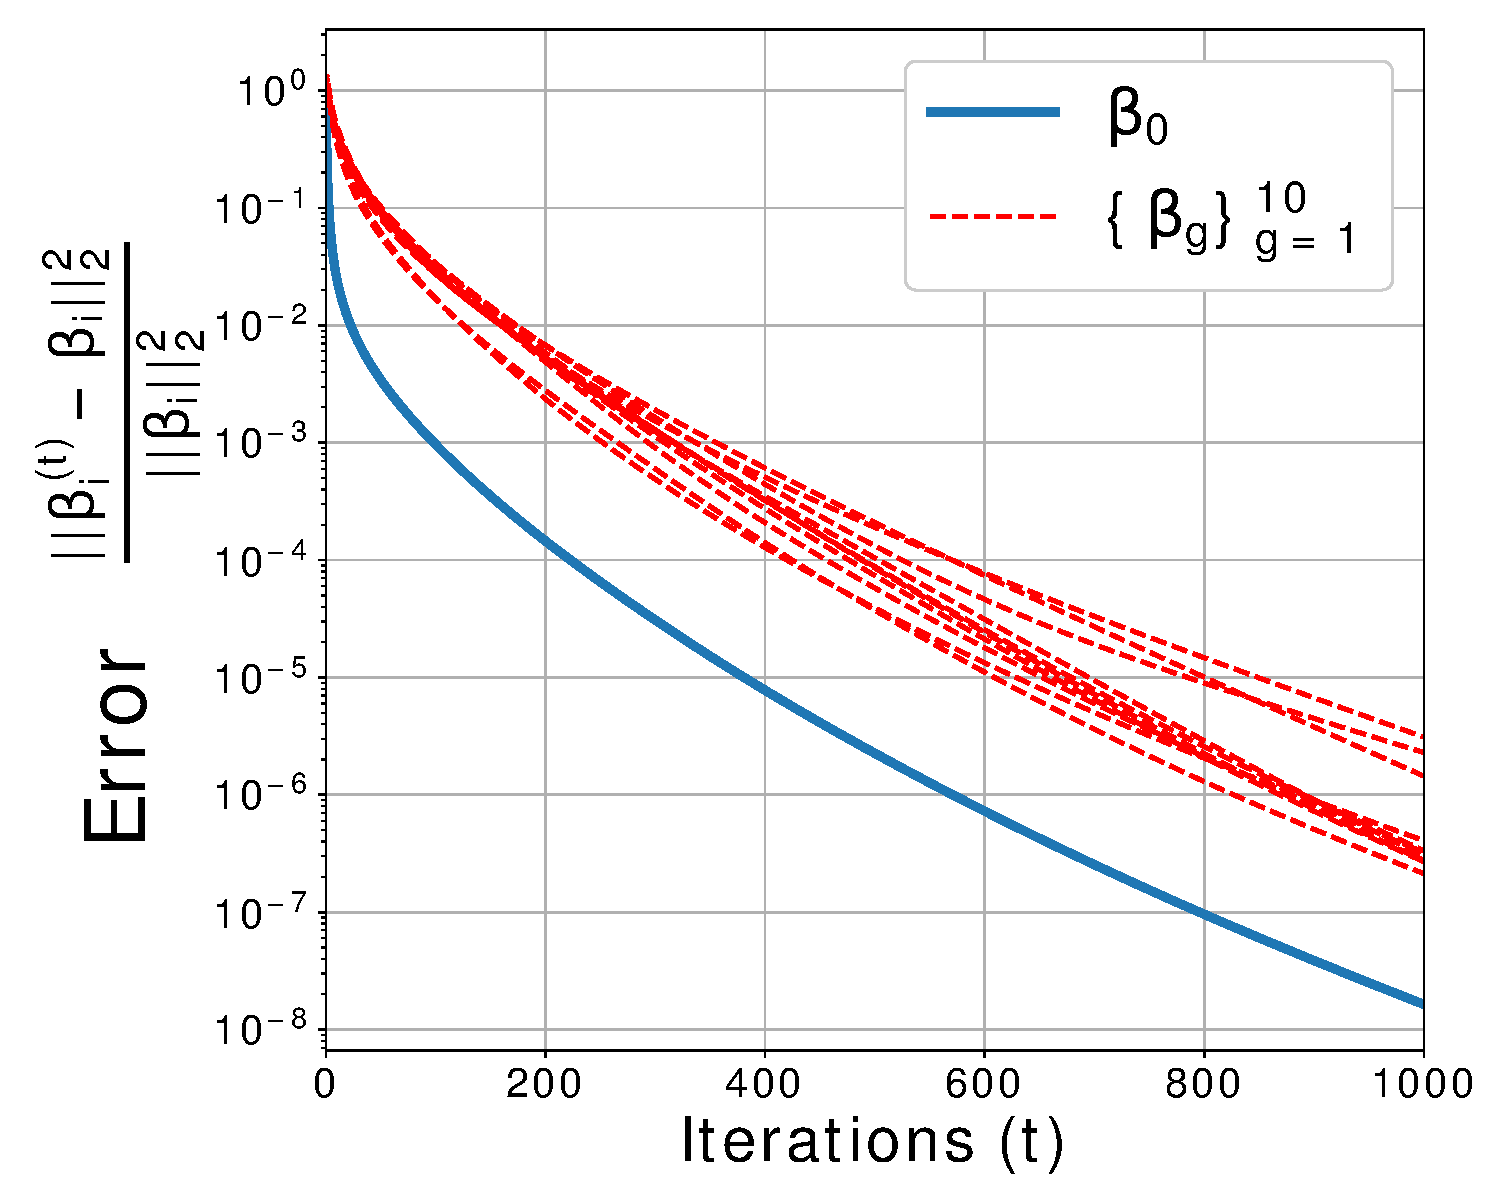
\includegraphics[width=\textwidth]{img/betag_converge_G10_p100.eps}
%			
%			\caption{}\label{fig syn1a}
%		\end{subfigure} ~
%		\begin{subfigure}[b]{0.5\textwidth}
%			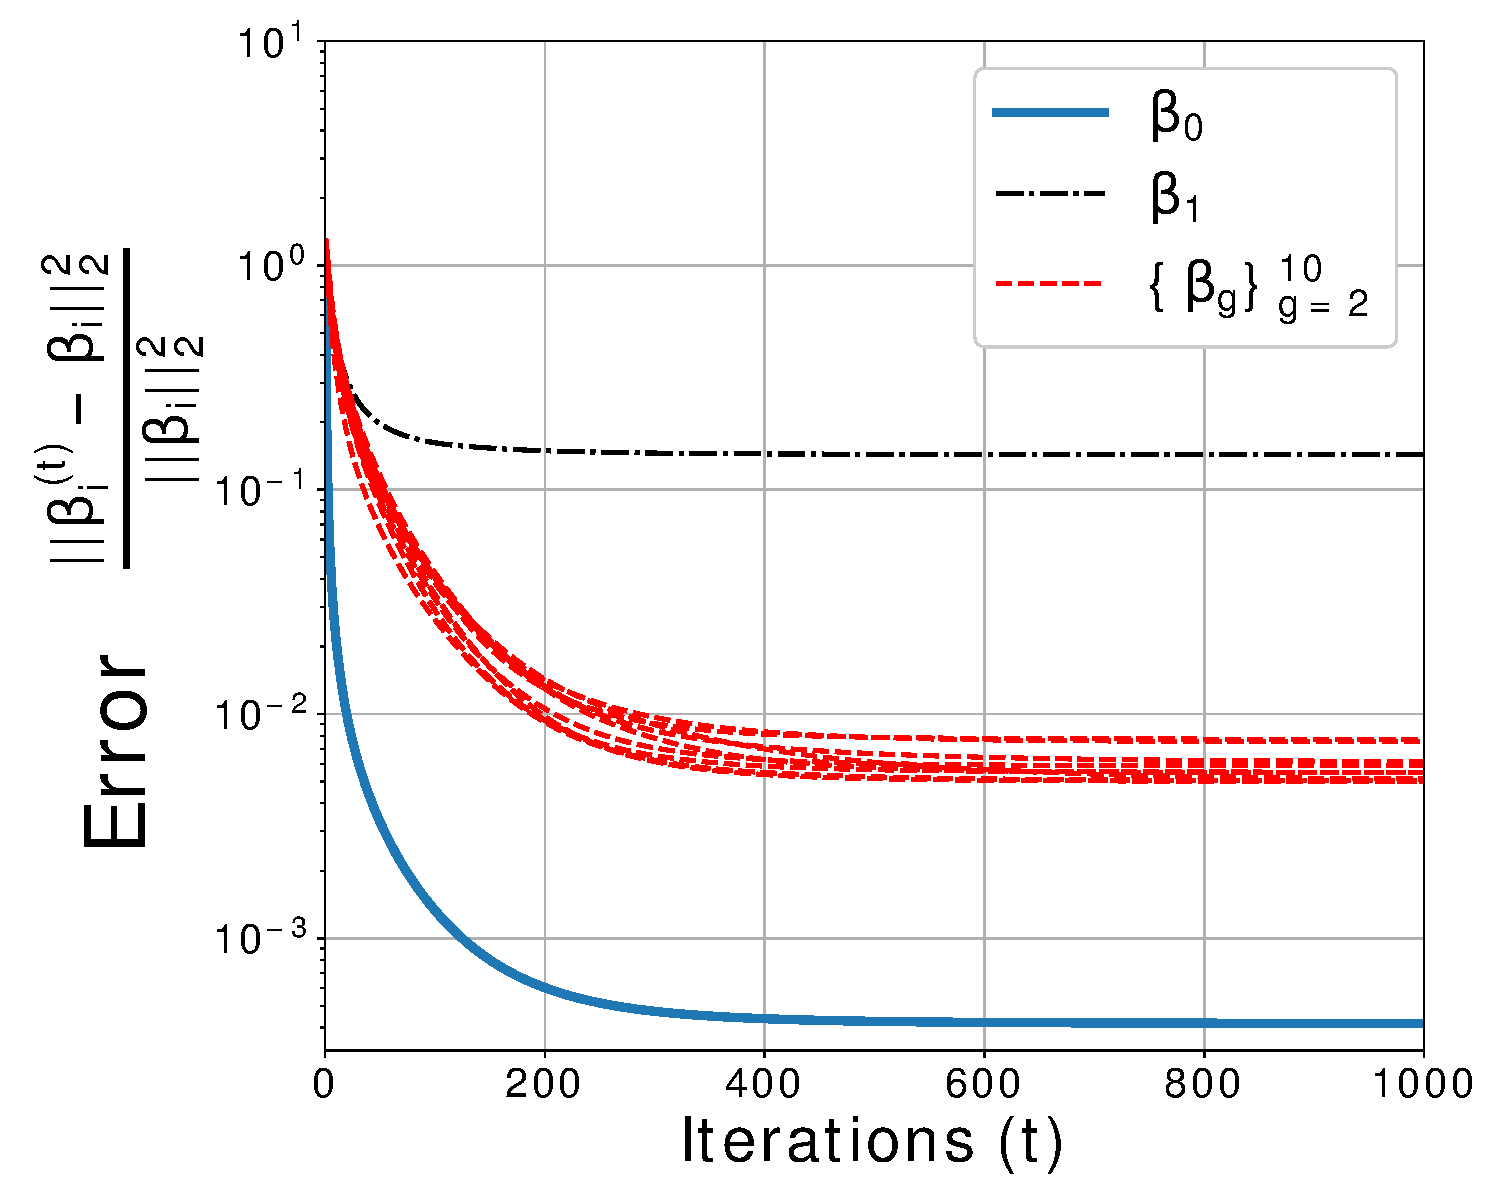
\includegraphics[width=\textwidth]{img/betag_converge_noise_G10_p100.eps}
%			
%			\caption{}\label{fig syn1b}
%		\end{subfigure}
%		\caption{a) Noiseless fast convergence. b) Noise on the first group does not impact other groups as much.}
%		\label{fig syn1}
%	\end{figure}
%	
%	\begin{figure}[t!]
%		\begin{subfigure}[b]{0.5\textwidth}
%			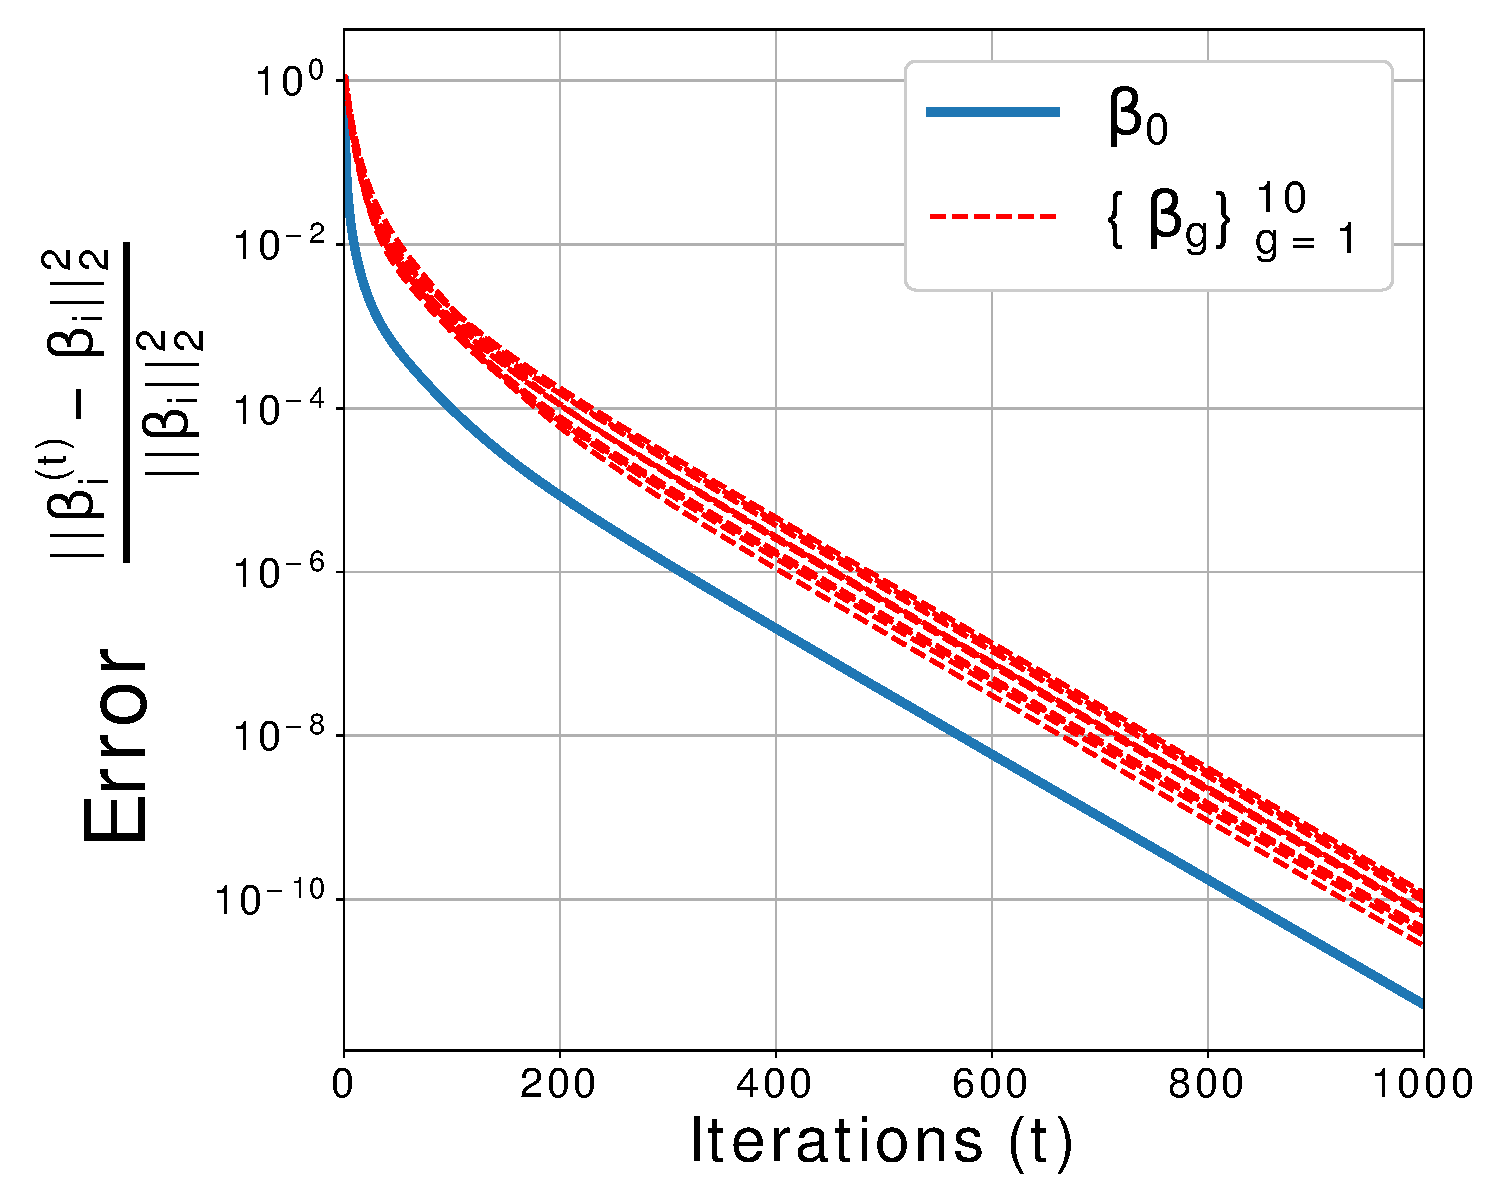
\includegraphics[width=\textwidth]{img/betag_converge_G10_p100_fast.eps}
%			
%			\caption{} \label{fig syn2a}
%		\end{subfigure} ~
%		\begin{subfigure}[b]{0.5\textwidth}
%			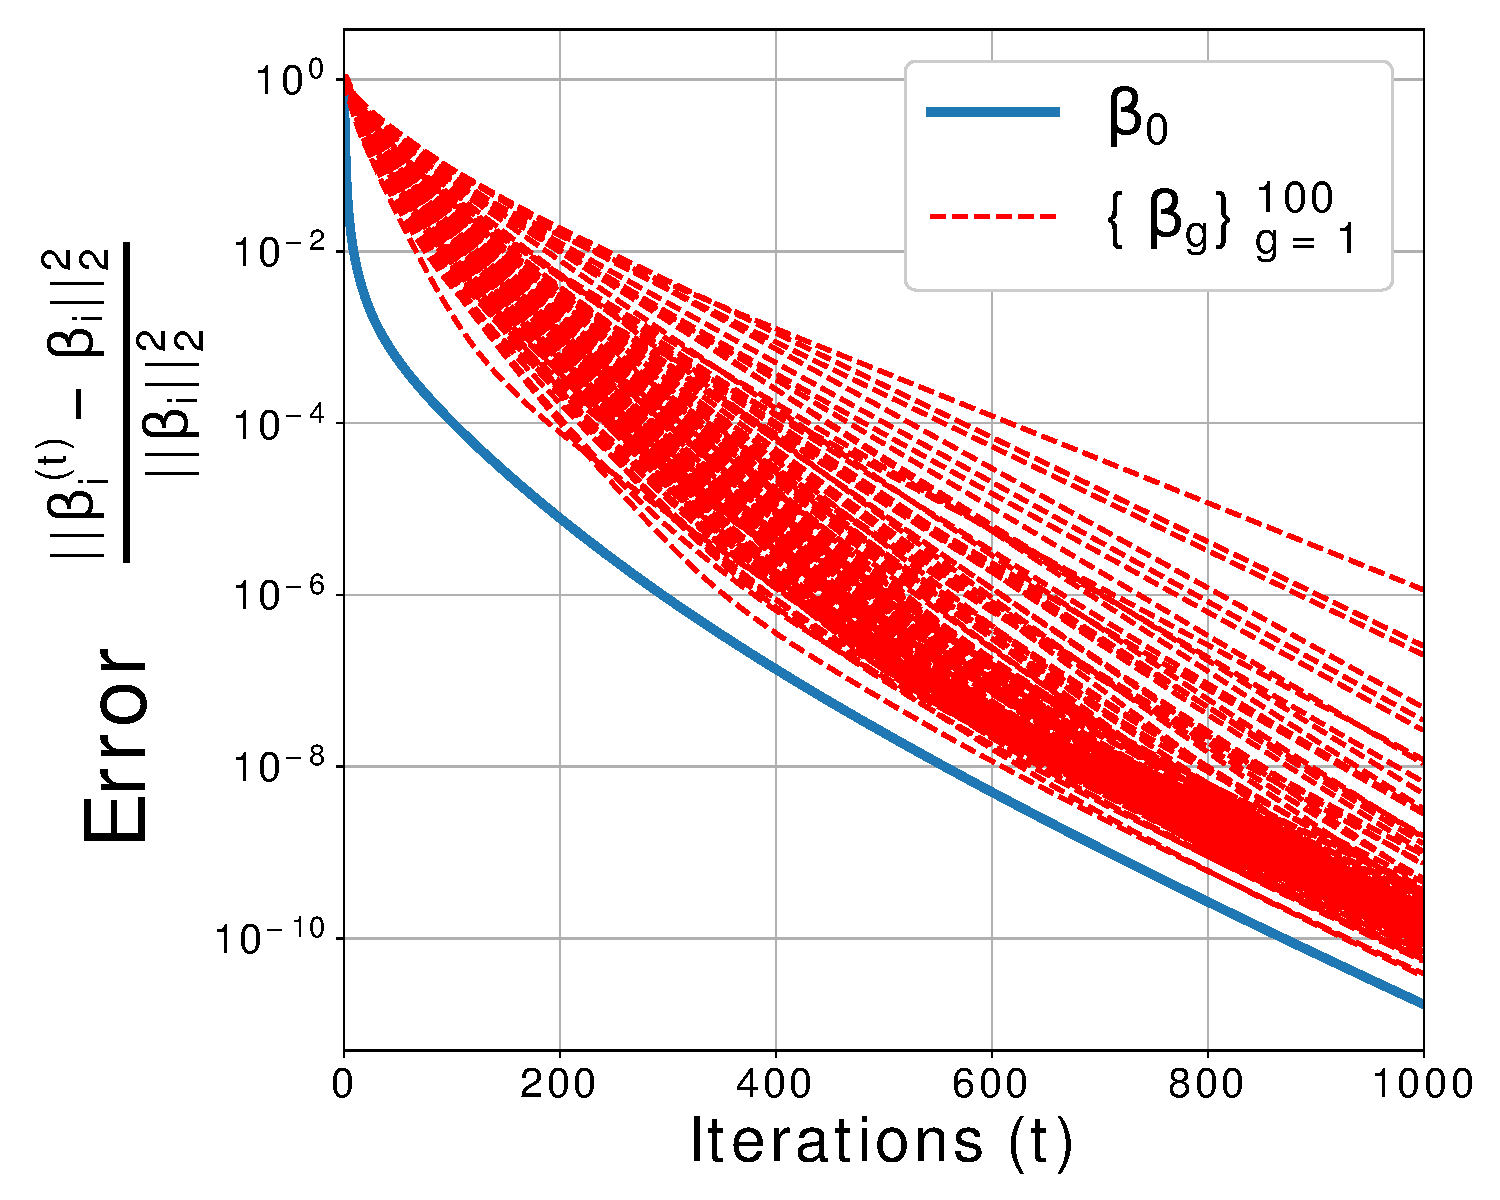
\includegraphics[width=\textwidth]{img/betag_converge_G100_p1000_shrink}
%			
%			\caption{}\label{fig syn2b}
%		\end{subfigure}
%		\caption{a) Increasing sample size improves rate of convergence. b) Our algorithm convergences fast even with a large number of groups $G=100$.}
%		\label{fig syn2}
%	\end{figure}



%%%%%%%%%%%%% Amir's exp commented for now
%In this section we supplement our theoretical results with a simple synthetic experiment. 
%We focus on the case of two groups, i.e., $G = 2$. 
%The dimension $p = 1000$ and the structure is sparsity induced by $l_1$-norm. 
%The parameters $\bbeta _0^*$, $\bbeta _1^*$, and $\bbeta _2^*$ are 20, 10, and 5-sparse respectively. 
%The sparsity pattern is as follows:$\bbeta _0^* = (\underbrace{1, \dots, 1}_{1-20}, 0, \dots)$,$\bbeta _1^* = (\dots, 0, \underbrace{2, \dots, 2}_{51-60}, 0, \dots)$, and $\bbeta _2^* = (\dots, 0, \underbrace{-2, \dots, -2}_{96-100}, 0, \dots)$. 
%
%For the distribution of input and noise we have $\x_{gi} \sim N(0, \sigma_x^2 \I)$ and $\omega_{gi} \sim N(0, \sigma_w^2)$ with $\sigma_x^2 = .3$ and  $\sigma_w^2 = .1$.
%We use the SPGD method (Algorithm \cref{alg2}) to solve the optimization problem \cref{eq:compact}. 
%The projection to the $l_1$ ball can be efficiently performed by the method proposed in \cite{dssc08}. 
%
%While changing $n$ in the experiments, we keep the ratio $\frac{n_1}{n_2} = \frac{2}{3}$ fixed. 
%Figures \cref{fig:individual1} and \cref{fig:individual2} show the per-group error for different sample size which follows $1/\sqrt{n_g}$ decay.
%Finally, Figure \cref{fig:common} shows the decay of the error as sample size increases for the common component recovery and the error for summation of the form \cref{eq:errorsum}.
%As expected errors decay as $1/\sqrt{n}$.
%
%\begin{figure}
%	\centering
%	\subcaptionbox{
%		Individual parameter one.
%		\label{fig:individual1}
%	}{\includegraphics[width=0.3 \textwidth]{./img/synthbeta1}}~
%	\subcaptionbox{
%		Individual parameter two.
%		\label{fig:individual2}
%	}{\includegraphics[width=0.3 \textwidth,]{./img/synthbeta2}}
%	\subcaptionbox{
%		Common parameter.
%	\label{fig:common}
%	}{\includegraphics[width=0.3 \textwidth,]{./img/synthbeta0}}
%	\caption{Estimation error with different sample size. Each point on the diagram is an average over 30 experiments.} %\cref{fig:common} compares the error with the LHS of \cref{eq:errorsum}
%	\label{fig:gasprices}
%\end{figure}


